

\subsection{Calibración}
\label{calibracion}

Para poder obtener la posición en tres dimensiones de los marcadores a partir de las imágenes capturadas es necesario que las cámaras estén previamente calibradas. El objetivo de la calibración consiste en determinar un conjunto de parámetros tal que pueda establecerse una relación entre el espacio 3D y las coordenadas 2D de las imágenes.\\

Los puntos en el espacio pueden ubicarse respecto a un sistema de coordenadas 3D. A su vez, los puntos capturados en las imagenes pueden referenciarse respecto a un sistema de coordenadas 2D en píxeles. Si se quiere determinar la posición de un punto en el espacio en función de las correspondientes proyecciones de dicho punto en las imágenes capturadas por las cámaras, es necesario determinar las ecuaciones que vinculan al sistema de coordenadas del espacio con el sistema de coordenadas en píxeles de las cámaras.\\

De la relación entre estos sistemas de coordenadas se obtienen los parámetros de las cámaras. Dichos parámetros se clasifican en intrínsecos y extrínsecos. Los primeros son aquellos que describen las propiedades geométricas y ópticas de la cámara, es decir, las características internas de la cámara. Por otra parte, los parámetros extrínsecos son los que describen la posición y orientación de la cámara respecto al sistema de coordenadas del espacio.\\

Para realizar esto es necesario establecer un modelo que describa el sistema de óptico de las cámaras. Esto es, el modelo por el cual una cámara es capaz de transformar el espacio 3D en imágenes de dos dimensiones. Un modelo simple y que describe estos sistemas adecuadamente es el modelo “pinhole” de las cámaras. 
El modelo "pinhole" se basa en la implementación mas simple de una cámara real, la cámara estenopeica.\\


El modelo de esta cámara se describe en la figura \ref{pinhole}.\\

\begin{figure}[hbt]
\begin{center}
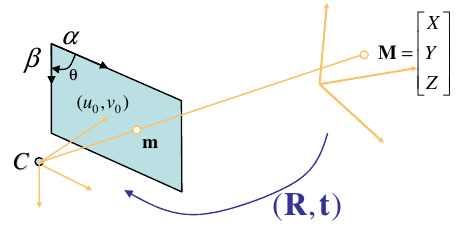
\includegraphics[scale=0.7]{img/calibracion/pinhole_camera.png}
\end{center}
\caption{Modelo "pinhole" de una cámara.}
\label{pinhole}
\end{figure}

En dicho modelo, una cámara se representa por un punto $C$, foco de la cámara, y un plano, al  que se le llama retina de la cámara. La imagen que se proyecta en la retina corresponde a la imagen capturada por la cámara. Dado un punto $M$ en el espacio, su correspondiente proyección en la retina, el punto $m$, se encuentra en la intersección de la retina y la recta formada por los puntos $C$ y $M$ de manera que $C$, $M$ y $m$ son colineales.\\










